;\chapter{Network Error Logging a relevantné technológie}
\label{nel-and-related-technologies}

% TODO:
% \begin{enumerate}
%     \item Zavolať s Petrom ohľadom predstavy, ako chcem napísať úvod o "Internete"
%     \item Naštudovať podklady k Report API LEPŠIE, aby som presne vedel čo chcem spomenúť
% \end{enumerate}


% POZNAMKY:

% the global system of interconnected computer networks
% Internet, a system architecture that has revolutionized mass communication, mass media, 
% and commerce by allowing various computer networks around the world to interconnect. Sometimes referred to as a “network of networks,”

% the world wide web is an information retrieval service of the web. It provides users with a huge array of documents that are connected to each other 
% by means of hypertext or hypermedia links. Here, hyperlinks are known as electronic connections that link the related data so that users can easily access 
% the related information hypertext allows the user to pick a word or phrase from text, and using this keyword or word or phrase can access 
% other documents that contain additional information related to that word or keyword or phrase. World wide web is a project which is created by Timothy Berner’s 
% Lee in 1989, for researchers to work together effectively at CERN. It is an organization, named World Wide Web Consortium (W3C), 
% which was developed for further development in the web.


% %##########################################################

% Príbeh kapitoly 2.:

% \# Prostredie                                 OK
% \# Identifikácia Komunikanta                  OK
% \# Komunikácia                                OK
% \# Obsah komunikácie                          OK
% \# Zobrazovanie a práca s obsahom             OK

% \# Aký problém vzniká
% Zlyhanie komunikácie
%     Dosiahnuteľnosť Web Serveru               
%     Bežné, detekovateľné (HTTP 400, 500)      
%     Nedetekovateľné (Elaborate pls)           

% \# Reporting API
% Reporting API                                 
%     Riešenie pre čo                           
%     Ako                                       
%     Nedostatky                                

% \# Subjekt analýzy    
% Network Error Logging                         
%     Stav Webu ???                             
%     Web Performance                           
%     SEO                                       

\todo{rewrite after this whole chapter is done}

Network Error Logging (ďalej už iba \textbf{NEL}) je technológia využívaná vo webovom prostredí, 
kde má svoju rolu v monitorovaní špecifických problémov komunikácie počítačových zariadení využívajúcich služby webu.
Pre dostatočné pochopenie, čím je technológia NEL, v tejto kapitole vysvetľujem najprv 
spomínané prostredie, v ktorom figuruje. 
Následne popíšem čo predstavujú pojmy monitorovanie a zlyhanie komunikácie na webe, kde zároveň popíšem body, v ktorých môžu rôzne zlyhania nastať. 
V prvom rade sa pri popise problematiky zameriavam na terminológiu, ktorá sa v nadchádzajúcich častiach tejto práce fekventovane používa. 
Samotný popis pre NEL nasleduje za úvodom do techológie, ktorá NEL spojazdňuje ako jeho závislosť, \textbf{Reporting API}, bez ktorej samostatne nemôže fungovať. % refs ?


\section{Webové prostredie}
\label{webove-prostredie}

V rámci internetu, globálnej infraštruktúry sieťou prepojených zariadení, ktorá tvorí takzvanú sieť sietí, existuje systém World Wide Web (ďalej už iba web).
Web je služba ponúkajúca možnosť získavať dokumenty uložené na internete, a teda na zariadeniach do neho pripojených, nazývaných taktiež \textbf{web server}. 
Vyhľadávanie a získavanie spomínaných dokumentov, a teda obsahu dostupného na web serveri, funguje na základe ich vzájomného prepojenia takzvanými hyperlinkami.
Termín \textbf{hyperlink} v tomto kontexte prestavuje taký odkaz na dokument, ktorý umožňuje tento dokument identifikovať, lokalizovať a získať z webu. 
Hyperlinky sa vyskytujú ako súčasti obsahu získavaného dokumentu, a to vo forme či už textu (\textbf{hypertext}) alebo rôznych iných typov médií (\textbf{hypermédiá}), ako napríklad obrázky, videá alebo reklamy. 


\begin{figure}[htb]
\begin{center}
 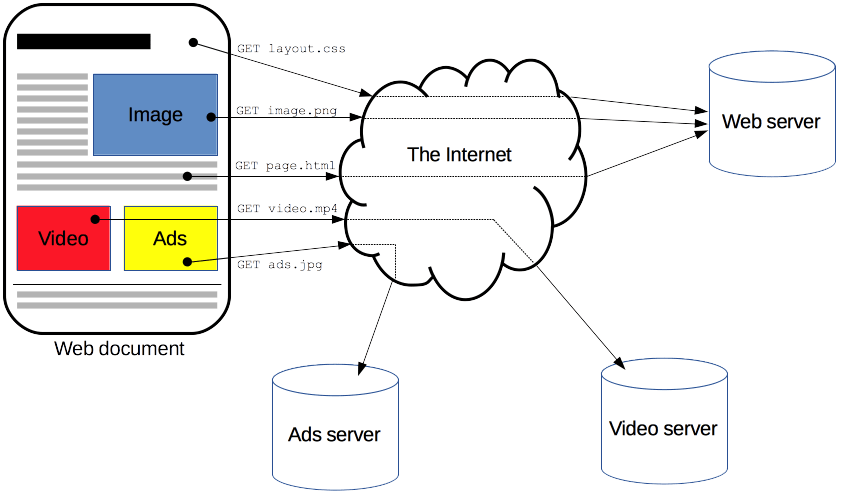
\includegraphics[scale=0.55]{obrazky-figures/fetching_a_page.png}
 \caption{\centering Vizualizácia webového prostredia. Za využitia infraštruktúry internetu prepája pomocou hyperlinkov dokumenty, ktoré možno na webe prehliadať.}
 \label{img:fetching-a-page}
\end{center}
\end{figure}

\todo{cite the images}

\pagebreak

\subsection{Štruktúra hyperlinku}
\label{navigacia-na-webe}

Hyperlinky na iné dokumenty sú formované ako reťazcová hodnota nazývaná Uniform Resource Locator (jednotný lokátor zdrojov, ďalej už iba \textbf{URL}).
Vďaka hyperlinkom obsahujúcim hodnoty URL je možné odkazovať sa na vzdialený obsah webu, prepájať rôzne dokumenty medzi sebou, a tým web navigovať.
Typická hodnota URL sa skladá z:
\begin{enumerate}
    \item adresy web servera, teda jeho domény (domény sú popísané v kapitole \ref{domeny})
    
    \item schémy - označenie \textbf{protokolu} používaného na sieťovú komunikáciu medzi servermi,
    
    \item a cesty k uloženému dokumentu.
\end{enumerate}

\begin{figure}[htb]
\begin{center}
 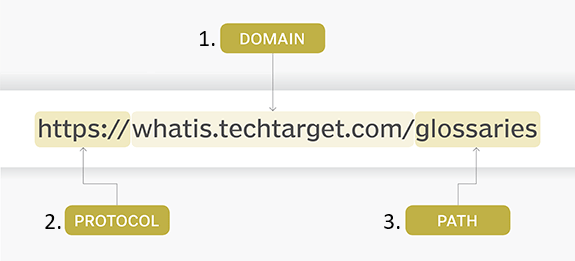
\includegraphics[scale=0.52]{obrazky-figures/the-anatomy-of-a-url.png}
 \caption{\centering Základná štruktúra hodnoty URL. Prvá časť (1.) označuje doménu web servera, druhá (2.) komunikačný protokol a tretia (3.) cestu k dokumentu. Hodnoty bývajú rôzne a môžu sa skladať z niekoľkých ďalších častí, no tie však nie je potrebné pre účely tejto práce rozoberať.}
 \label{img:urlstructure}
\end{center}
\end{figure}

\pagebreak

Tieto hlavné zložky hodnôt URL predstavujú samostatne dôležité koncepty pre navigáciu vo webe.
Protokol (2.) definuje možinu platných pravidiel pre komunikáciu zariadenia návštevníka webu s web 
serverom, ktorého prislúchajúce meno je definované ďalšou časťou URL --- doménou (1.). 
Cestu k uloženému dokumentu (3.) web server interpretuje podľa jeho konfigurácie ako navigačné inštrukcie 
v rámci jeho vlastného, alebo vzdialeného úložiska jemu sprístupneného. 
Podľa týchto inštrukcií vyberie server vyžiadaný dokument a zašle ho naspäť spomínanému návštevníkovi webu.
V ďalších kapitolách tento proces postupne opisujem detailnejšie.

\subsection{Domény}
\label{domeny}

Pre adresovanie počítačových zariadení na internete sa používa adresa \textbf{IP}.
Takáto adresa môže mať dve podoby:
\begin{enumerate}
    \item IPv4, napríklad \code{192.0.2.172},
    \item IPv6, napríklad \code{2001:db8:8b73:0000:0000:8a2e:0370:1337}.
\end{enumerate}

\todo{TCP/IP pouziva IP adresy a stara sa o session}
Pomocou takýchto adries taktiež funguje navigácia na internete, označovaná pojmom smerovanie správ v komunikácií medzi počítačmi.
Popis funkcionality smerovania správ nie je dôležitý pre oblasť záujmu tejto práce, no dôležitým faktom je, že \textbf{smerovanie dokumentov vo webovom prostredí funguje na základe smerovania správ pomocou IP adries}.

Vo webovom prostredí však prenášané dokumenty môžu byť uložené na nespočetne veľkom počte počítačových zariadení.
Jednou nepriaznivou skutočnosťou je, že IP adresa web serveru poskytujúceho nejaký dokument sa môže časom meniť.
Ďalej, pre návštevníkov webu je nepraktické pamätať si zložité IP adresy pre dokumenty, ktoré chcú vyhľadať.

Z týchto dôvodov sa zaviedlo používanie \textbf{doménových mien}, ktoré predstavujú mená priradené adresám IP v systéme nazvanom Domain Name System (\textbf{DNS}, systém doménových mien), ktorý ich spravuje.
Využitím systému DNS je teda možné v hodnotách URL namiesto zložitých cieľových IP adries používať doménové mená k nim priradené.  

\subsubsection{Systém doménových mien}

DNS je distribuovaný systém doménových mien prislúchajúcich k IP adresám počítačových zariadení na internete.
Na skladovanie a spravovanie týchto mapovaní používa DNS špecifické databáze pre svoj systém. 
Jeho primárnou službou je vyhľadávanie IP adries podľa spomínaných doménových mien.
Táto služba sa nazýva \textbf{DNS rezolúcia} (anglicizmus, pojem sa do slovenčiny doslovne neprekladá). 
O vykonávanie rezolúcií sa stará program nazvaný \textbf{DNS rezolver} (rovnako, anglicizmus).
Proces pridania IP adresy do systému DNS \mbox{s jej} novým doménovým menom sa nazýva \textbf{registrácia}.
Registrácia môže byž vykonaná:
\begin{itemize}
    \item buď \textbf{registrantom} -- majiteľom zariadenia s IP adresou,

    Registrant vytvára žiadosť o registráciu doménového mena (napríklad na stránkach registrara).

    \item alebo \textbf{registrarom}.

    Registrar je správca a poskytovateľ služieb DNS v jemu pridelenej zóne tohto systému. % ?
    Pri registráciach TLD je bežne vykonávateľom samotej registrácie registrar. % ?
\end{itemize}

% rfc8499 pages 2,15,
% https://developer.mozilla.org/en-US/docs/Glossary/DNS

\subsubsection{Štruktúra doménového mena}

Ako bolo zmienené, doménové meno je textová hodnota reprezentujúca adresu webového serveru.
Doménové meno sa rozdeľuje na viaceré úrovne nazývané levely. 
Jednotlivé levely sú v ňom oddelené znakmi bodky. 
Level najviac vpravo v doménovom mene sa nazýva \mbox{\textbf{TLD} -- Top Level Doména}. 
Ďalší level smerom doľava (predposledná hodnota) spolu s TLD tvorí \mbox{\textbf{SLD} -- Secondary Level Domain}.
Posledný level spolu s SLD a TLD vytvára SD -- \textbf{subdoménu}.

V doménovom mene \code{example.domain.com} platí rozdelenie nasledovne: 
\begin{itemize}
    \item \code{\underline{example}.domain.com} predstavuje celé meno subdomény,
    \item \code{\underline{domain}.com} predstavuje celé meno SLD,
    \item \code{\underline{.com}} predstavuje TLD.
\end{itemize}

Každá časť oddelená bodkou má v rámci celkového doménového mena svoj vlastný názov a logický význam.
Kompozícia doménového mena však v určitých prípadoch nemusí byť jednotlivými bodkami rozdelená na vyššie popísané levely. 
Túto skutočnosť popisuje nasledujúci \mbox{obrázok \ref{fig:domain-name-structure}}, \mbox{ktorý} berie v úvahu doménové meno skladajúce sa až z piatich bodkou oddelených častí.

\begin{figure}[htb]
\begin{center}
 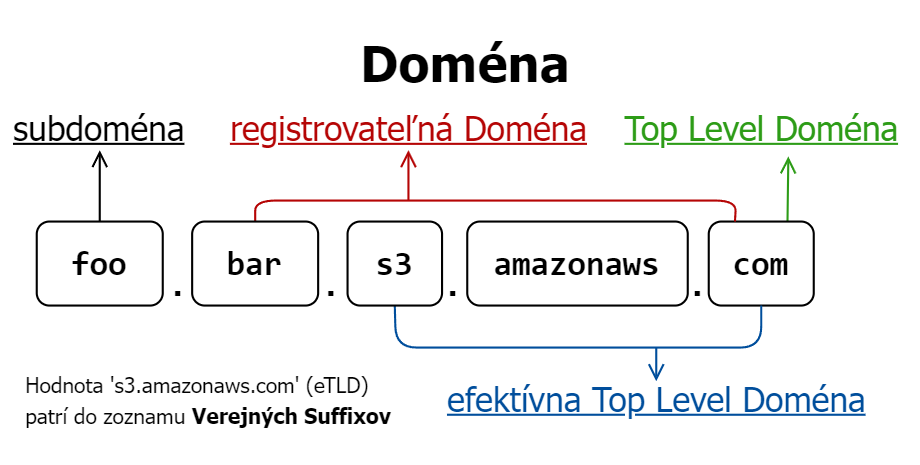
\includegraphics[scale=0.45]{obrazky-figures/domain_name_structure.png}
 \caption{\centering Príklad domény s nezvyčajnou štruktúrou. Postupným skladaním hodnôt oddelených bodkou začínajúc \mbox{z pravej} strany vznikajú logické časti mena domény. V tomto prípade ide o výnimku, pri ktorej neplatí, že čiastkové hodnoty oddelené bodkou predstavujú jej jednotlivé levely \mbox{(viď definíciu termínu \textbf{Verejný Suffix} nižšie).}}
 \label{fig:domain-name-structure}
\end{center}
\end{figure}


\subsubsection{Verejný Suffix a eTLD}

Doménové meno popisované obrázkom \ref{fig:domain-name-structure} --- \code{foo.bar.s3.amazonaws.com} --- sa ako každé iné doménové meno skladá z TLD, SLD a subdomény. 
Platia tu však niektoré ďalšie dôležité pravidlá pri ich identifikovaní.

Existuje zoznam nazývaný \textbf{Public Suffix List} (zoznam verejných suffixov, skratka \textbf{PSL}), v ktorom sa nachádzajú koncovky doménových mien, pod ktorými je možné registrovať domény a subdomény pre web servery.
Tieto koncovky uvedené v PSL sa nazývajú efektívne Top Level Domény (\textbf{eTLD}).
Hodnoty eTLD zahŕňajú vyššie spomínané TLD ako ich podslednú bodkou oddelenú hodnotu.
Preto je pri celých menách registrovaných domén vhodnejšie rozdeľovať ich na eTLD, SLD (meno registrovanej domény) a subdoménu.

S použitím hodnoty eTLD '\code{s3.amazonaws.com}' vybranej z PSL je možné rozdeliť doménové meno z obrázka \ref{fig:domain-name-structure} na jeho levely nasledovne: 
\begin{itemize}
    \item \code{\underline{foo}.bar.s3.amazonaws.com} predstavuje celé meno subdomény,
    \item \code{\underline{bar}.s3.amazonaws.com} predstavuje celé meno SLD -- registrovanú doménu,
    \item \code{\underline{s3.amazonaws.com}} predstavuje eTLD, kde \code{.com} je TLD.
\end{itemize}

% https://www.michalspacek.com/origin-site-etld-etld-plus-one-public-suffix-psl-what-are-they

Na záver chcem ako poznámku uviezť, že sa môže pre označenie domény eTLD vyskytovať aj výraz rovnakého významu -- Pay Level Domain (PLD, preložiteľné so zachovaním významu ako doména zakúpiteľného levelu).

\subsection{Protokol HTTP}
\label{protokol-http}
\todo{prepisat za pouzitia terminologie domen}
\\
Definíciou, v oblasti sietí termín protokol predstavuje štandardizovanú množinu pravidiel pre vzájomnú komunikáciu medzi počítačovými zariadeniami. % \ref{}
Vzhľadom na to, že funkčnosť technológie NEL sa zakladá na komunikácií za pomoci protokolu HTTPS, % \ref{}
venujem sa v tejto sekcií výhradne protokolom HTTP a jeho zabezpečenej, uvedenej verzii --- HTTPS. 

% \ref{https://www.rfc-editor.org/rfc/rfc9110.html}
HTTP, celým názvom HyperText Transfer Protokol, je bezstavový aplikačný protokol pre distribuované hypertextové informačné systémy. 
Poskytuje jednotné komunikačné rozhranie pre prenos dokumentov (daľej v terminológií špecifikácie HTTP už iba ako \textbf{zdroj}).
Toto rozhranie definuje dva typy zasielateľných správ --- \textbf{žiadosť} a \textbf{odpoveď}. Žiadosť predtavuje doslova žiadosť o zdroj. Odpoveď je reakciou na žiadosť, kde je možné, že sa navráti buď žiadaný zdroj, alebo popis chyby, ktorá vznikla pri pokuse o jeho navrátenie. 

Protokol funguje na základe klient-server komunikácie, kde klient a server sú názvy rolí, ktoré môžu prepojené zariadenia zaujať v rámci komunikácie pomocou HTTP:
\begin{itemize}
    \item \textbf{Klient} zakladá spojenie so serverom za účelom zasielania jednej alebo viacerých \mbox{žiadostí}. 
    
    Program implementujúci komunikačné rozhranie pre rolu klienta sa nazýva tiež \textbf{User Agent} (skrátene UA, slovensky -- agent používateľa). Pre bežného návštevníka webu ako UA \mbox{figuruje} \textbf{webový prehliadač} nainštalovaný na jeho zariadení. Webovým prehliadačom sa viac venuje kapitola \ref{webovy-prehliadac}.
    
    \item \textbf{Server} prijíma spojenia aby obslúžil žiadosti tým, že na ne zasiela prislúchajúce odpovede.

    Pre program implementujúci rozhranie takéhoto servera sa používa označenie \textbf{Origin Server} (server pôvodu zdroja, ďalej ako \textbf{origin}).
    
\end{itemize}

\begin{figure}[htb]
\begin{center}
    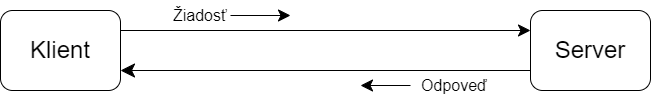
\includegraphics[scale=0.6]{obrazky-figures/http-client-server.png}
    \caption{\centering Vizualizácia konceptu komunikácie pomocou protokolu HTTP. Klient zasiela požiadavku na server a server mu naspäť posiela odpoveď.}
    \label{fig:http-client-server}
\end{center}
\end{figure}

\pagebreak

\subsubsection{HTTP žiadosť}

\begin{figure}[htb]
\begin{center}
    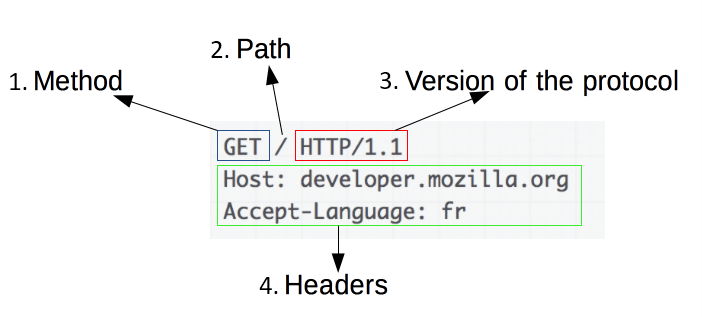
\includegraphics[scale=0.6]{obrazky-figures/http_request.png}
    \caption{\centering Príklad HTTP žiadosti. Jednotlivé časti požiadavky sú na obrázku označené číslami. Postupne, prvá časť (1.) predstavuje metódu žiadosti, nasleduje cesta \mbox{k zdroju (2.)}. Ďalšia je vyznačená verzia protokolu HTTP (3.), pod ktorou je v poslednom rade umiestnená sekcia s HTTP hlavičkami (4.).}
    \label{fig:http-request}
\end{center}
\end{figure}

Správy HTTP protokolu sú štruktúrované bloky textu.
Správa nadväzujúca HTTP spojenie, teda žiadosť, má nasledovný obsah:
\begin{enumerate}
    \item Metóda žiadosti

    Metóda žiadosti indikuje operáciu, ktorú klient chce aplikovať na žiadaný zdroj.
    Podľa metódy server zistí, aký výsledok úspešne aplikovanej operácie očakáva klient v odpovedi.

    Dôležité metódy sú najmä:
    \begin{itemize}
        \item GET --- klient žiada zdroj v jeho aktuálnom stave. 
        \item POST --- klient chce vykonať špecifický proces s obsahom, ktorý pridá k žiadosti. 
        Bežne sa jedná napríklad o nahranie nového zdroju z klienta na server.
    \end{itemize}
    
    \item Cesta k požadovanému zdroju

    Jedná sa tu o cestu spomínanú v kapitole \ref{navigacia-na-webe}, bod 3. v popise príkladnej URL (viď obrázok \ref{img:urlstructure}).
    Cesta môže byť symbolická, teda určená pre interpretáciu samotným serverom (podľa jeho konfigurácie) ako napríklad \code{/glossaries}, alebo priamo označujúca konkrétny zdroj, napríklad \code{/glossaries.txt}.  
 
    \item Verzia protokolu HTTP použitého na nadviazanie a priebeh komunikácie
    
    \item Sekcia polí s ďalšími informáciami a nastaveniami komunikácie --- \textbf{HTTP Headers}
    
    Táto hovorovo nazývaná sekcia \textbf{hlavičiek} obsahuje páry názvov polí a ich priradených hodnôt. 
    Hlavičky slúžia ako definície možností a iných potrebných informácií pri komunikácií medzi zariadeniami.
    Pre názvy hlavičiek existuje register \textit{Hypertext Transfer Protocol (HTTP) Field Name Registry},
    v ktorom sa uvádzajú oficiálne hlavičky použiteľné pri komunikácií HTTP. 

    Príkladom potrebnej informácie pre HTTP žiadosť je hlavička \code{Host}, ktorej hodnota musí reprezentovať doménu cieľového web servera. 
    
    \item Prípadný obsah žiadosti

    Napríklad obsah pridaný k žiadosti s metódou POST. 
    Obsah sa pridáva pod sekciu HTTP hlavičiek, od ktorej sa oddeľuje práznym riadkom (znakmi \code{\textbackslash r\textbackslash n}).

    \item Zakončenie správy --- dva prázdne riadky (znaky \code{\textbackslash r\textbackslash n\textbackslash r\textbackslash n})

\end{enumerate}


\subsubsection{HTTP odpoveď}

\begin{figure}[htb]
\begin{center}
    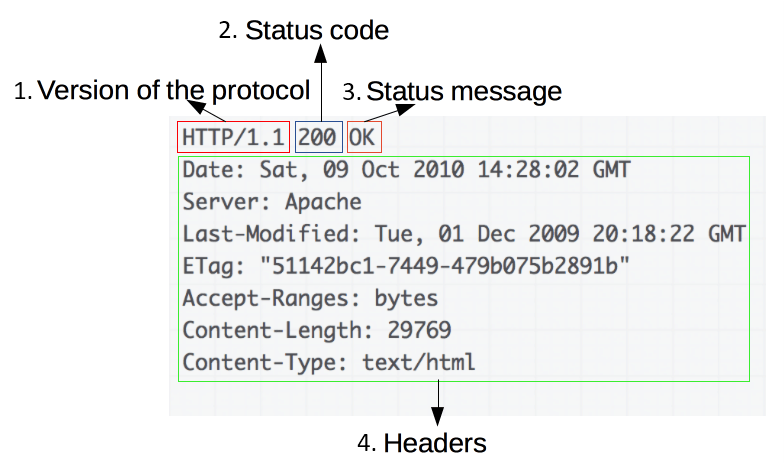
\includegraphics[scale=0.6]{obrazky-figures/http_response.png}
    \caption{\centering Príklad HTTP odpovede. Jednotlivé časti odpovede sú na obrázku označené číslami. Prvú časť (1.) tvorí verzia protokolu HTTP, za ňou sa nachádza \mbox{statusový kód (2.)} a správa k nemu prislúchajúca (3.). Pod nimi je na konci odpovede umiestnená sekcia s HTTP hlavičkami (4.). Väčšinou býva k odpovedi pridaný aj dodatočný obsah, ktorý by nasledoval ako časť oddelená prázdnym riadkom od hlavičiek.}
    \label{fig:http-response}
\end{center}
\end{figure}

\noindent HTTP odpoveď sa od žiadosti mierne líši. Obsahuje nasledovné časti:

\begin{enumerate}
    \item Verzia protokolu HTTP použitého na odsoslanie odpovede

    \item Statusový kód reprezentujúci výsledok vykonanej operácie vyvolanej HTTP žiadosťou

    Takýto kód v je v odpovedi reprezentovaný ako trojciferné celé číslo, ktoré môže popisovať jeden
    zo stavov rozdelených do piatich kategórií podľa ich významu. 
    Kategórie významov sú určené prvou číslicou čísla statusového kódu, ktoré môže nadobúdať hodnoty od 1 po 5:

    \begin{enumerate}
        \item 1xx (info)
        
        Status tohto typu s hodnotami od 100 do 199 indikuje predbežné odpovede určené pre komunikáciu stavu pripojenia (v komunikácií HTTP) alebo stavu priebehu spracovania prislúchajúcej žiadosti.
        Odpovede so statusom 1xx sa zasielajú predtým ako sa dokončí operácia vyžiadaná žiadosťou a zašle sa pre ňu finálna odpoveď.
        
        \item 2xx (úspech)
        
        Statusy 2xx s hodnotami od 200 do 299 oznamujú klientovi, že jeho žiadosť bola úspešne prijatá, spracovaná a akceptovaná. 
        
        \item 3xx (presmerovanie)
        
        Status 3xx indikuje, že pre dokončenie obsluhy žiadosti klienta musí klient vykonať ďalšiu alebo inú akciu.
        V odpovedi obsahujúcej presmerovanie sa teda nachádza nový zdroj, ktorý by mal klient vyžiadať, aby mohla byť dokončená obsluha jeho pôvodnej žiadosti. 
        Statusy tejto kategórie môžu nadobúdať hodnoty od 300 do 399.
        
        \item 4xx (chyba klienta)

        Status chyby klienta s hodnotami od 400 do 499 oznamuje klientovi, že sa vyskytol problém s jeho žiadosťou.
        Server teda zasiela klientovi odpoveď, v ktorej vysvetľuje chybu v jeho žiadosti.
        
        \item 5xx (chyba servera): The server failed to fulfill an apparently valid request

        Hodnoty 500 až 599 označujú problémy, ktoré vznikli na strane servera jeho vlastným zapríčinením, alebo zapríčinením jeho závislostí (databáza, sieťové operácie a podobne).
        Server, ktorý odošle odpoveď so statusom z tejto kategórie oznamuje klientovi, že jeho žiadosť nemôže byť obslúžená, pretože pri obsluhe server zlyhal.
    \end{enumerate}

    \item Správa prislúchajúca k statusovému kódu

    Ku každému statusovému kódu prislúcha nejaká popisná správa sformovaná ako obyčajný reťazec zakončený ASCII znakom pre nový riadok. Správy sú šdandardizované ako frázy spísané v anglickom jazyku.
    Medzi najbežnejšie statusové správy podľa statusových kódov patria:

    \begin{itemize}
        \item \code{100} -- \code{CONTINUE}: Server pokračuje v spracovávaní žiadosti,
        \item \code{200} -- \code{OK}: Žiadosť úspešne spracovaná,
        \item \code{301} -- \code{MOVED PERMANENTLY}: Zdroju bola priradená iná URL,
        \item \code{404} -- \code{NOT FOUND}: Zdroj sa nenašiel,
        \item \code{500} -- \code{INTERNAL SERVER ERROR}: Server pri obsluhe žiadosti zlyhal.
    \end{itemize}

    \pagebreak

    \item Sekcia s hlavičkami

    Táto sekcia je štruktúrovaná rovnako ako v HTTP žiadosti. V prípade odpovede sem však naviac pribúdajú ďalšie hlavičky, ktoré by odpoveď mala zahŕňať: 

        \begin{itemize}
            \item \code{Date}: dátum a čas odoslania odpovede
            \item \code{Server}: software nainštalovaný na web serveri (origin server), ktorý odpoveď zaslal
            \item \code{Content-Length}: dľžka obsahu odpovede v bajtoch
            \item \code{Content-Type}: typ média prenášaného v obsahu odpovedi

            Hodnota typu média musí byť jedným s registrovaných názvov typov v zozname \textit{Multipurpose Internet Mail Extensions} (MIME). Príkladmi MIME typov pre prenášaný obsah sú hodnoty \code{text/plain} pre obyčaný text, \code{text/html} pre HTML alebo \code{image/png} pre obrázky.
        \end{itemize}

    \item Obsah odpovede

    Pre umiestnenie obsahu v odpovedi platí to isté ako pre obsah umiestnený v žiadosti.
\end{enumerate}


\subsubsection{HTTPS}

Dáta spomínané v sekciách o žiadosti a odpovedi sa prenášajú v HTTP komunikácií ako obyčajný text. 
Tým pádom v prípade odpočúvania a potencionálneho pokusu o ovplyvnenie tejto komunikácie má tretia strana (útočník) prístup k všetkým prenášaným dátam. 
To znamená, že útočník následne môže dáta z komunikácie čítať, pozmeniť alebo pridať svôj vlastný obsah. 
Je teda nutné ochrániť komunikáciu klienta so serverom pred pred nežiadúcimi zásahmi z tretej strany.

Z toho dôvodu bol vyvinutý protokol HTTPS - Secure (bezpečný) HTTP.
HTTPS je zabezpečená verzia protokolu HTTP, ktorá šifruje všetky prenášané dáta medzi klientom a serverom.
V kontextoch senzitívnych operácií vykonávaných na webe, ako napríklad prenos súkromných dokumentov, poskytuje HTTPS bezpečný spôsob vymienňania dát so serverom.

O samotné šifrovanie v rámci prenosu HTTPS sa stará protokol TLS -- Transport Layer Security (bezpečnosť prepravnej verstvy).
TLS je rovnako ako HTTP protokol pre komunikáciu klienta so serverom a jeho použitím pri komunikácií HTTP sa spojenie medzi zariadeniami zabezpečuje proti odpočúvaniu, manipulácií a falšovania správ. 

% https://httpwg.org/specs/rfc7230.html, https://httpwg.org/specs/rfc7231.html

\subsection{Obsah hľadaných dokumentov}
\label{obsah-hladanych-dokumentov}

Webové dokumenty, alebo iným použitý pomenovaním -- webové zdroje, sa prenášajú v prostredí webu pomocou protokolu HTTP (viď obrázok \ref{img:fetching-a-page}).
Tieto dokumenty sú buď získané samostatne ako jednotlivé súbory (textový súbor, obrázok, archív \code{.zip}), alebo ako zoskupená množina viacerých súborov v podobe webovej stránky.

\textbf{Webová stránka} (skrátene \textbf{webstránka}) je typ dokumentu, ktorého obsahom je hypertext alebo hypermédiá štruktúrované vo formáte \textbf{HTML}.
HTML je formát webového dokumentu skladajúceho sa z počiatočnej definície typu dokumentu a stromovej štruktúry takzvaných elementov, kde prvým je element \code{<html>}. 
Jednotlivé elementy sa do HTML súboru vpisujú pomocou značiek, pričom, okrem jednotlivých výnimiek, 
každý element musí mať otvárciu (\code{<elementXY>}) a zatváraciu značku (\code{</elementXY>}).
Vnútorne sa HTML delí na dve hlavné sekcie --- \textbf{hlavičku} pre metadáta dokumentu a \textbf{telo} pre jeho vnútorné rozpoloženie a obsah.
Elementy môžu mať k sebe priradené položky uchovávajúce ich doplnkové detaily nazývané atribúty. 
Napríklad element používaný pre vytvorenie hyperlinku s názvom \code{\textbf{<a>}} (anglicky skratka pre \textit{anchor}) 
môže mať priradený atribút s názvom \code{\textbf{href}} obsahujúci URL odkazovaného dokumentu.

\begin{center}
\centering
\begin{lstlisting}[caption={\centering Základná štruktúra HTML dokumentu. HTML obsahuje počiatočnú definíciu typu dokumentu (\code{<!DOCTYPE html>}), hlavičku, telo, hyperlink a popisné komentáre.},
label=listing:html-struktura, 
language=HTML, 
frame=tb,
xleftmargin=.05\textwidth, 
xrightmargin=.05\textwidth]
    <!DOCTYPE html>
    <!-- %*Toto je komentár, ktorý sa na stránke klientovi nezobrazí*) -->
    <html lang="sk">       
        <!-- %*HTML hlavička*) -->
        <head>
         <title>%*Príklad HTML dokumentu*)</title>
        </head>
        <!-- %*HTML telo*) -->
        <body>
         <!-- %*Ukážka vytvorenia hyperlinku: element <a> a jeho atribút href*) -->
         <a href="https://google.com">%*Hypertext odkazujúci na stránku google*)</a>
        </body>
    </html>
\end{lstlisting}
\end{center}

Vo výpise \ref{listing:html-struktura} súbor HTML tvorí štruktúru iba pre odkaz na vzdialenú webstránku.
Pridať rôzne, už spomínané hypermédiá ako obrázky, audio a video (ale aj dokumenty HTML), je však možné vďaka dvom ďalším kategóriam elementov. 
Sú nimi: 
\begin{enumerate}
    \item Elementy \code{<link>} patriace do hlavičky HTML.

    Tieto elementy odkazujú na vzdialené metadáta pre samotnú webstránku.
    Typ metadát udáva atribút s názvom \code{rel}, ktorý môže nadobúdať napríklad hodnotu 
    \code{'author'} alebo \code{'help'} pre vytvorenie odkazu na autora stránky, alebo dokumentu poskytujúcemu 
    pomocný manuál pre obsah stránky.
    
    \item Elementy obsahujúce atribút \code{src} patriace do tela HTML.

    Akýkoľvek element z tejto kategórie môže odkazovať na podporovaný typ hypermédia, 
    ktorý udáva názov takéhoto elementu.
    Pre spomínané typy hypermédií ide o elementy: 
    \begin{itemize}
        \item \code{<img>} -- obrázky,
        \item \code{<audio>} -- audiosúbory,
        \item \code{<video>} -- videá,
        \item \code{<iframe>} -- HTML dokumenty, ktoré možno vnoriť do ich referujúcej webstránky.
    \end{itemize}
    
\end{enumerate}

Každé samostatné hypermédium, ktoré tieto elementy označujú je potrebné získať ako zdroj ďalšou HTTP žiadosťou spolu so samotnou stránkou, ktorá na toto hypermédium odkazuje.

\subsection{Webový prehliadač}
\label{webovy-prehliadac}

\todo{search engine}
% https://developer.mozilla.org/en-US/docs/Glossary/Search_engine
% http://infolab.stanford.edu/%7Ebackrub/google.html

Softvér, ktorý slúži na navigovanie webu --- získavanie zdrojov na webe --- stavaný ako implementácia HTTP klienta, teda ako UA (User Agent) sa nazýva \textbf{webový prehliadač}. 
Tým, že je prehliadač implementáciou HTTP klienta (viď kapitolu \ref{protokol-http}), dokáže zasielať žiadosti a spracovávať odpovede HTTP.
Je to teda program, ktorý využíva koncepty vysvetlené vyššie a je schopný prehľadávať web.

Používateľ s nainštalovaným prehliadačom má možnosť vyhľadávať zdroje či už podľa 
kľúčových slov, ktoré obsahujú, alebo podľa špecifických URL na ne odkazujúcich.
Prehliadač získané zdroje buď ukladá na úložisku zariadenia (jednoduché zdroje ako archív \code{.zip}), alebo, v prípade, že ide o zdroj reprezentujúci webstránku, ju po získaní zobrazuje.  

Webstránky sú v prehliadači vybudované a zobrazené podľa ich obsahu HTML (viď kapitolu \ref{obsah-hladanych-dokumentov}).
Na uskutočnenie tohto procesu vybudovania a zobrazenia webstránky používa prehliadač svoje zabudované algoritmy.
Moderné webstránky okrem samotného zdroja HTML obsahujú aj prídavné závislé zdroje, ktoré môžu priamo danej webstránke upraviť vzhľad alebo pridať programovateľnú funkcionalitu.
Prehliadač takéto zdroje získava pomocou odkazov, ktoré sú definované v hlavičke alebo tele dokumentu HTML prislúchajúceho danej webstránke.
Rovnako ako pre proces zobrazovania HTML má prehliadač zabudované algoritmy aj pre prácu so zdrojmi tohto typu.

V tejto práci je dôležité popísať konkrétne zdroje pridávajúce programovateľnú funkcionalitu.
Sú nimi zdroje obsahujúce prehliadačom spúšťateľné skripty napísané v programovacom jazyku \textbf{JavaScript}.

\subsubsection{JavaScript}
\label{javascript}

Jazyk JavaScript multiplatformový programovací jazyk, ktorého využitím je v oblasti webu práve robiť webstránky interaktívnymi. 
Jedným z jeho využití je manipulácia so stromovou štruktúrou obsahu HTML dokumentu (viď kapitolu \ref{obsah-hladanych-dokumentov}).
Funkcionalita zabezpečujúca podporu pre takúto manipuláciu s obsahom webstránok a ďalšie podobné funkcionality sú v jazyku JavaScript dostupné ako \textbf{Web API}.

API\footnote{API -- Application Programming Interface (programové rozhranie aplikácie)} predstavuje predprogramovaný balík kódu, ktorý uľahčuje jeho používateľom, teda programátorom, prácu v oblasti zamerania funkcionality daného balíka.
Ďalej, skutočnosť, že ide o webové API znamená, že je možné taký balík využiť prostredníctvom JavaScriptu spojeného s webstránkou.
Existuje množstvo webových API, z ktorých niektoré sú poskytované priamo prehliadačom používateľa webu, iné zasa tvorcami tretej strany (Third-party API).

% https://developer.mozilla.org/en-US/docs/Learn/JavaScript/Client-side_web_APIs/Introduction

\subsubsection{JavaScript Object Notation}
\label{json}

V spojení s konceptami jazyka JavaScript vznikol jeden konkrétne dôležitý textový formát dát s názvom \textbf{JSON} -- JavaScript Object Notation.
Štruktúra formátu JSON je jednoduchá a je založená na niektorých dátových typoch jazyku JavaScript.
Dokáže reprezentovať nasledovné dátové typy:
\begin{enumerate}
    \item primitívne: reťazce, čísla, pravdivostné hodnoty (boolean) a absenciu hodnoty (null)
    \item štruktúrované: polia (array) a objekty

    Pole je usporiadaná sekvencia 0 a viac hodnôt. 
    \\
    Objekt je neusporiadaná kolekcia 0 a viac párov kľúč--hodnota, kde kľúč je reťazec
    a hodnota môže byť akýkoľvek primitívny alebo štruktúrovaný dátový typ.
    
\end{enumerate}

JSON má využitie napríklad ako formát dát pri komunikácií typu HTTP na webe.
\mbox{V správach}, ktoré obsahujú zdroj typu JSON musí byť nastavená HTTP hlavička s názvom \code{Content-Type} na hodnotu typu MIME \code{application/json}.

\begin{center}
\centering
\begin{lstlisting}[caption={\centering Príklad dokumentu JSON. Položka \code{"student"} predstavuje JSON kľúč, ktorého hodnotou je štruktúrovaný dátový typ objekt. Názornú ukážku dátového typu pole predstavuje hodnota priradená kľúču \code{"predmety"}.},
label=listing:priklad-dokumentu-json, 
language=json, 
frame=tb,
xleftmargin=.15\textwidth, 
xrightmargin=.15\textwidth]
    {       
        "student": {
            "login": "xjurik12",
            "kredity": 162,
            "predmety": ["ITT", "IBP"],
            "vyborny_priemer": false
            "diplom": null
        }
    }
\end{lstlisting}
\end{center}

% JSON spec = https://www.rfc-editor.org/rfc/rfc7159

\section{Monitorovanie zlyhaní webstránok}

Cieľom tejto práce je analyzovať technológiu spojenú s monitorovaním zlyhaní v komunikácií 
na webe --- Network Error Logging (NEL).
Technológie, na ktorých sa NEL zakladá alebo ich používa, boli vysvetlené v predošlej kapitole \ref{webove-prostredie}.
Ďalej už popisujem termíny spojené priamo s NEL.

\subsection{Monitorovanie}
\label{monitorovanie}

Pojem monitorovanie webstránok je na verejne dostupných zdrojoch definovaný ako proces testovania a kontrolovania či používateľ webu, konkrétne danej webstránky, môže s ňou pracovať tak, ako to očakáva jej poskytovateľ. 

Keďže sa venujem monitorovaniu v kontexte s technológiou NEL, webstránku možno zameniť za akýkoľvek zdroj uložený na webe.
Poskytovateľ, teda správca webového serveru, kde sa zdroj nachádza, používa monitorovanie pre získanie informácií ohľadom jeho dostupnosti alebo zlyhaniach pri jeho získavaní.
Tento proces býva automatizovaný tak, že monitorovací nástroj zaznamenáva žiadosti o získanie zdroja a na zistené zlyhania upozorňuje jej poskytovateľa.  
Vďaka aplikovanému monitorovaniu teda správca web serveru nadobúda prehľad o stave dostupnosti ním spravovaných zdrojov.

% Toto nie je to prave orechove :(
% https://en.wikipedia.org/wiki/Website_monitoring

\pagebreak

\subsection{Body zlyhania}

Proces prehliadania webu môžme definovať ako získavanie vzdialených zdrojov, ako napríklad webstránok, použitím webového prehliadača.
Za predpokladu, že používateľ má dostupnú adresu URL pre zdroj (viď kapitolu \ref{navigacia-na-webe}), 
ktorý chce získať, má tento proces nasledovnú postupnosť úkonov na vykonanie:

\begin{enumerate}
    \item prehliadač získa adresu IP pre doménu web serveru z danej URL v systéme DNS,
    
    \item prehliadač vytvorí so zariadením adresovaným získanou IP adresou spojenie protokolom TCP 
    (pojmy DNS a TCP/IP z kapitoly \ref{domeny}),
    
    \item prehliadač použije spojenie TCP s web serverom na zasielanie HTTP žiadostí 
    (popísaných v kapitole \ref{protokol-http}) s cieľom získať zdroj uvedený v danej URL.
\end{enumerate}

Každý z vyššie uvedených krokov môže skončiť s nejakou chybou, teda neúspešne, čo by spôsobilo celkové zlyhanie procesu získania cieľového zdroja.
Na základe týchto troch potrebných krokov pre úspešné získanie zdroja možno rozdeliť zlyhania do troch kategórií:
\begin{enumerate}
    \item zlyhania komunikácie s DNS,

    Tieto zlyhania môžu zahŕňať nedostupnosť DNS servera, chybové odpovede bez nájdenej 
    IP adresy web servera so zdrojom alebo iné neočakávané zlyhania ako napríklad náhle prerušenie spojenia s DNS serverom.
    
    \item zlyhania nadviazania spojenia TCP/IP,

    Spojenie s webovým serverom, na ktorom je zdroj uložený, môže zlyhať pri:
    \begin{itemize}
        \item zakladaní spojenia,
        
        Adresa IP servera je neplatná, server je nedostupný alebo spojenie neprijal
        
        \item náhlom ukončení spojenia,

        Server môže spojenie uzavrieť, resetovať, alebo skrátka prerušiť.  

        \item alebo pri zakladaní bezpečného spojenia (HTTPS),

        Komunikácia pomocou zabezpečeného protokolu HTTPS, ako už bolo spomínané, využíva na zabezpečenie základnej verzie HTTP protokol nazvaný TLS.
        V jednoduchosti, TLS spojenie sa vytvorí, iba ak sú pre také spojenie splnené požiadavky na ako webového klienta, tak aj webový server. 
        Zlyhania zakladania TLS spojenia môžu nastať pri rôznych prípadoch nesplnenia týchto požiadavok. 
        Pre referenciu sú takéto prípady vymenované v kapitole o NEL, 
        N-KAPITOLY% \ref{nel} 
        , pod sekciou s preddefinovanými zlyhaniami pre monitorovanie NEL.
        
    \end{itemize}
    
    \item a zlyhania prenosu HTTP.

    Za zlyhanie sa v rámci prenosu HTTP považuje:
    \begin{itemize}
        \item zlyhanie samotného protokolu,

        Napríklad môže programovo zlyhať softvér pre HTTP origin server (chyba v implementácií origin servera).
        HTTP odpoveď môže byť nesprávne skonštruovaná, napríklad, keď obsahuje konfliktné hodnoty hlavičiek a obsahu (hodnota hlavičky \code{Content-Length} nesedí so skutočnou dĺžkou obsahu).  
        Ešte však dochádza aj k situáciam, pri ktorých sa vytvorí takzvaný \textit{redirect loop}, čo predstavuje slučku presmerovaní HTTP klienta. Takáto slučka spôsobuje, že klient neustále zasiela tú istú sekvenciu žiadostí, no nikdy sa nedopracuje k cieľovému zdroju.
        
        \item ale aj úspešná HTTP odpoveď so statusom z kategórie 4xx, alebo 5xx.

        Odpovede so statusom 5xx reprezentujú zlyhanie na strane origin servera, ktorý nebol schopný poskytnúť vyžiadaný zdroj.
        Naopak, odpovede so statusom 4xx sú chybami na strane klienta. 
        Avšak, aj tieto chyby sú z hľadiska monitorovania vzácne, pretože nadmerne časté opakovanie takejto chyby môže pomôcť odhaliť nesprávne zadefinované (alebo jednoducho zastarané a neudržované -- status 404) hyperlinky na webstránke správcu, ktorý ju monitoruje. 
    \end{itemize}
    
\end{enumerate}

\section{Network Error Logging}
\label{network-error-logging}

Podľa definície monitorovania z kapitoly \ref{monitorovanie}, NEL slúži ako mechanizmus
zabezpečujúci monitorovanie zlyhaní žiadostí pre zdroje uložené na web serveri, ktorý NEL používa.
Predtým však, ako sa dostanem k popisu NEL, jeho možnostiam a konfigurácii, musím popísať konkrétnu Web API -- Reporting API, na ktorej je z hľadiska svojej funkcionality závislý.

\subsection{Závislosť na Reporting API}
\label{reporting-api}

Reporting API je jedným z balíkov označovaných názvom Web API (viď kapitolu \ref{javascript}).
Serverom, ktoré Reporting API používajú, poskytuje možnosť definovať pravidlá pre 
tvorbu a zasielanie takzvaných hlásení na pravidlami definované web servery.
Hlásenia sa týkajú špecifických záležitostí prehliadača klienta, ktorý žiada zdroje z web serveru používajúceho Reporting API.
Medzi takéto špefifické funkcie patrí práve NEL, ale napríklad aj detegovanie výskytov zlyhaní alebo používania zastaraných API na klientskom prehliadači.

Aby bolo možné tento balík uplatniť, musí ho podporovať webový prehliadač (konkrétne User Agent) používateľa, ktorý zasiela žiadosti o získanie zdrojov zo servera využívajúceho Reporting API.

\subsubsection{Verzia používaná technológiou NEL}

V tomto bode je dôležité povedať, že aj keď je najnovšou verziou tejto API verzia popisovaná špecifikáciou zverejnenou 10. novembra 2023, v tejto kapitole nepopisujem práve túto.
Dôvodom je, že technológia NEL je stále v procese vývoja a jej momentálna verzia je implementovaná tak, aby fungovala so staršou verziou Reporting API.
Konkrétne, NEL je kompatibilný s verziou popisovanou v špecifikácií zverejnenej 
25. septembra 2018, taktiež označovanou ako verzia \textbf{\code{v0}}.
Ďalej teda opisujem výhradne Reporting API verzie \code{v0}.

\subsubsection{Definícia pravidiel}

Vyššie spomínané pravidlá môže definovať server, ktorý chce využívať tento API balík. 
Definícia pravidiel funguje prostredníctvom zaslania HTTP hlavičky \code{Report-To} v HTTP odpovedi pre vybraný zdroj.
Obsahom hlavičky \code{Report-To} musí byť textová hodnota vo formáte JSON (viď kapitolu \ref{json}), pričom jej štruktáru tvorí striktne pole (array) objektov.

Špecifickým rozdielom od klasického JSON formátu však je, že sa táto hodnota do hlavičky
zapisuje bez zátvoriek, ktoré bežne tvoria JSON pole (znaky '\code{[}' a '\code{]}').
S touto odchýlkou od bežného JSON formátu môže User Agent pracovať vďaka tomu, že pre takto špecifický formát existuje samostatný typ MIME s názvom \code{application/reports+json}. 

\pagebreak

Každý objekt v poli hodnôt hlavičky \code{Report-To} predstavuje pravidlo Reporting API.
Pravidlá sa musia ukladať v pamäti User Agenta, ktorému je odpoveď s pravidlami zaslaná.
Hodnota každého pravidla obsahuje nasledovné polia: 

\begin{enumerate}

    \item \code{group}

    Pole obsahujúce textový názov skupiny web serverov prislúchajúcich k danému pravidlu.
    
    Ak pravidlo neobsahuje toto pole, názov jeho skupiny web serverov bude \code{"default"}.
    
    \item \code{endpoints}

    Povinné pole \code{endpoints} musí definovať zoznam web serverov, ktoré patria do skupiny \code{group} (alebo skupiny \code{"default"}).
    Hodnota tohto poľa musí byť pole (array) JSON objektov s nasledovným obsahom:
    \begin{enumerate}
        \item \code{url} -- URL adresa konkrétneho web servera (povinná hodnota)
        \item \code{priority} -- Číslo definujúce prioritu servera v rámci skupiny \code{group}

        Priorita servera predstavuje jeho prednosť pred ostatnými v procese výberu servera, ktorému bude odoslané vygenerované hlásenie.
        
        \item \code{weight} -- Číslo určujúce prioritu serverov s rovnakou prioritou

        Tu priorita zase predstavuje prednosť servera pred ostatnými pri nerozhodnosti v prípade, že majú viaceré servery priradené rovnakú hodnotu \code{priority.}
    \end{enumerate}
    
    \item \code{max\_age}

    Ďalšie povinné pole definujúce životnosť daného pravidla. Jeho hodnotou musí byť nezáporné číslo reprezentujúce sekundy.

    Špeciálnym prípadom hodnoty tohto poľa je číslo \code{0}. 
    V prípade, že server pre pravidlo prislúchajpce konkrétnej skupine \code{group} vyplní \code{max\_age} hodnotou \code{0}, pravidlo stráca platnosť a musí byť vymazané.
    
    \item \code{include\_subdomains}

    Toto pole obsahuje pravdivostnú hodnotu \code{true} alebo \code{false}, podľa ktorej určuje či sa toto pravidlo platiace pre jeho skupinu \code{group} vzťahuje, a teda má používať, aj pre subdomény web servera, ktorý pravidlo zaslal.

    Ak nie je pole uvedené, pravidlo pre skupinu \code{group} sa nebude vzťahovať aj na subdomény.
    
\end{enumerate}

\begin{center}
\centering
\begin{lstlisting}[caption={\centering Príklad obsahu hlavičky \code{Report-To}. Pravidlo tu definuje skupinu s názvom \code{reporting-skupina}, ku ktorej prislúchajú dva web servery, kam môžu byť hlásenia zasielané s rozdielnou prioritou. Doba platnosti pravidla je 2 592 000 sekúnd, teda 30 dní.},
label=listing:priklad-report-to, 
language=json, 
frame=tb,
xleftmargin=.04\textwidth, 
xrightmargin=.04\textwidth]
    Report-To: {
        "group": "reporting-skupina",
        "endpoints": [
            {"url": "https://example.com/reporting1", "priority": 1},
            {"url": "https://example.com/reporting2", "priority": 2}
        ],
        "max_age": 2592000
    }
\end{lstlisting}
\end{center}


\subsubsection{Tvorba hlásení}

Počas doby platnosti aspoň jedného pravidla Reporting API existujúceho v pamäti 
User Agenta sa na ňom tvoria už spomínané hlásenia.
Hlásenie je správa týkajúca sa jednej z hlásiteľných udalostí, ktoré môžu nastať v prostredí prehliadača implementujúceho daný User Agent.
Medzi tieto hlásiteľné udalosti patrí: 
\begin{itemize}
    \item Prehliadač použije Web API, ktorá bola označená ako zastaraná
    \item User Agent sa rozhodol nezaslať ďalšiu žiadosť na Origin Server z bezpečnostných dôvodov
    \item Prehliadač zlyhal a bol terminovaný
    \item Došlo k zlyhaniu týkajúceho sa \textbf{oblasti monitorovania NEL}
\end{itemize}

\subsubsection{Zasielanie hlásení}

Nahromadené hlásenia sa periodicky odosielajú na web server cieľovej skupiny \code{group} pravidla vybraný podľa jeho priority.
Špecifikácia verzie \code{v0} Reporting API nedefinuje túto periódu odosielania sama, ale prenecháva túto zodpovednosť na prehliadače, ktoré sa rozhodnú API podporovať.

Ďalej, skupín \code{group} je práve toľko, koľko existuje uložených pravidiel s definovaným menom s zarátaním prípadnej skupiny \code{"default"}.
Výber cieľovej skupiny spočíva v ďalšom nastavení súvisiacim s Reporting API --- priradenie typu hlásenia k skupine.
Pre rôzne typy hlásení sa toto nastavenie zavádza inak.
V prípade hlásenia zlyhania v oblasti monitorovania NEL sa skupina \code{group} vyberá v samotnom nastavení pre NEL, ktoré priamo spolupracuje s pravidlami Reporting API.
Tento proces je popísaný v špecifikácií NEL, a to kapitole \ref{network-error-logging-spec}.

Hlásenia sú nahromadené a čakajú na odoslanie.
Každé z nich sa odošle vo formáte JSON na vybraný prioritný web server v nasledujúcej štruktúre:
\begin{itemize}
    \item \code{type} -- typ hlásenia

    Hodnoty môžu byť napríklad \code{crash} alebo \code{nel}.
    
    \item \code{age} -- vek hlásenia

    Vek hlásenia je čas v milisekundách, ktorý uplynul od jeho vytvorenia webovým prehliadačom.
    Podla implementacie podpory pre Reporting API môže webový prehliadač nechať nahromadiť viaceré hlásenia a zasielať ich oneskorene.
    
    \item \code{url} -- hodnota URL adresujúcej zdroj pre ktorý sa hlásenie vygenerovalo.

    Pripomínam, že hlásenia sa generujú pre akýkoľvek zdroj získaný z domény web servera, 
    ktorý definuje v jeho odpovedi pravidlá pre Reporting API.
    
    \item \code{user\_agent} -- názov a info o User Agentovi používateľovho webového prehliadača
    
    \item \code{body} -- telo hlásenia

    Telo hlásenia je vyplnené pre každý typ hlásenia inak. 
    V kapitole \ref{network-error-logging-spec}, kde sa priamo popisuje NEL je príklad hlásenia typu NEL na \todo{obrázku}.
    Najjednoduchší typ hlásenia je z pohľadu obsahu tohto poľa hlásenie o zlyhaní webového prehliadača.
    Taký typ hlásenia vyzobrazuje obrázok \ref{listing:priklad-generated-report}.
\end{itemize}


\begin{center}
\centering
\begin{lstlisting}[caption={\centering Príklad obsahu zaslaného hlásenia pre zlyhanie webového prehliadača. Hlásenie bolo odoslané 42 milisekúnd po jeho vytvorení na prehliadači Mozilla. Vygenerované bolo chybou, ktorá nastala po získaní zdroja prislúchajúceho k URL \code{https://example.com}. \mbox{Telo hlásenia} obsahuje ID zlyhania a ako dôvod je uvedená hodnota \code{oom}, ktorá reprezentuje chybu \textit{Out Of Memory} (nedostatok pamäte).},
label=listing:priklad-generated-report, 
language=json, 
frame=tb,
xleftmargin=.085\textwidth, 
xrightmargin=.085\textwidth]
{
  "type": "crash",
  "age": 42,
  "url": "https://example.com/",
  "user_agent": "Mozilla/5.0 (X11; Linux x86_64; rv:60.0) Gecko/20100101 Firefox/60.0",
  "body": {
    "crashId": "30437694edfeae5b",
    "reason": "oom"
  }
}
\end{lstlisting}
\end{center}

% TODO Asi si tu zamienam pojmy prehliadac a user agent
% TODO compatibility table

\subsection{Špecifikácia NEL}
\label{network-error-logging-spec}

% Security - https://www.w3.org/TR/secure-contexts/
% Dosiahnuteľnosť Web Serveru
% Web Reliability
% Možnosť definovať custom error typy

% Mail od Polcaka - Nieco naviac o NEL
% Consider - https://w3c.github.io/reporting/network-reporting

NEL, podobne ako Reporting API, je mechanizmus spúšťaný tým, že je User Agentovi pri žiadosti o cieľový zdroj v HTTP odpovedi zaslaná hlavičku \code{NEL}.
Hlavička \code{NEL} môže obsahovať jedno a viac pravidiel určených pre User Agenta, ktorý ak NEL podporuje, vyberie prvé správne sformované pravidlo v poradí a uloží si ho ako konfiguráciu NEL.
Ostatné pravidlá má User Agent podľa špecifikácie ignorovať.

Spolu s uvedenou hlavičkou s obsahom predstavujúcim konfiguráciu tejto technológie web server musí taktiež posielať klientovi hlavičku \code{Report-To}. 
Použitím NEL a Reporting API v tandeme zabezpečuje jednak nastavenie samotného monitorovania NEL, ale aj jeho závislosti -- tvorby a zasielania NEL hlásení.
User Agent, ktorý získal obe hlavičky začne generovať hlásenia o zlyhaniach týkajúcich sa prenášaných zdrojov medzi klientom a web serverom, z ktorej \code{NEL} hlavička bola odoslaná. 

Definovaných pravidiel môže byť viac ako jedno. 
Každé pravidlo však prislúcha jednej doméne priradenej web serveru a prípadne aj jeho subdoménam.

% Jako posiela reporte
% Jako vybera pravidlo
% Ako proces konci

% Zaslana hlavicka NEL
% Telo vygenerovaneho reportu (odkaz na Reporting API)
% Priklad
% Typy reportov
% Dodatocne vyhlasenia
% HOTOVINKO


% \section{OLD CONTENT}
% V tejto kapitole popisujem problematiku, v ktorej sa táto práca venuje. Jedná sa tu o možné nástrahy pri komunikácií typu klient-server,
% ktoré môžu nastať a spôsobiť probmlémy ako napríklad nedosiahnuteľnosť servera, s ktorým klient komunikáciu pôvodne nadviazal.
% O takýchto a podobných problémoch sa server ziaľ nemá ako dozvedieť, a preto vzniká potreba nájsť nejaký spôsob ako takéto problémy pri ich
% vzniku identifikovať a nahlásiť formou štruktúrovanej správy vývojárom zodpovedným za prevádzku daného servera. V prípade, že 
% na problém takto poukázané, v nasledujúcich krokoch je možné postaviť sa k nemu s vhodnými protiopatreniami a úspešne ho odstrániť, a teda 
% tak zároveň aj znovuspojazdniť predtým nefunkčnú komunkikáciu s klientami, u ktorých sa tento problém prejavoval.
% \\
% V tejto kapitole začnem s úvodom do širšieh spektra zavedenej problematiky, kde spomeniem technológie s podobným účelom 
% ako Network Error Logging (ďalej označovaný iba ako NEL), aké nedostatky aktuálneho stavu problematiky riešia, no hlavne, aké majú nedostatky. 
% Tým sa prepracujem k podstate a motivácií k nasadeniu samotného NEL-u a ďalších technológií priamo súvisiacich s ním. 
% Jedná sa tu čisto o teoretický základ nutný pre pochopenie nasledujúcich sekcií tejto práce. 
% Aktuálny stav využívania technológií spomínaných nižšie bude uvedený a detailne rozpísaný v kapitole \ref{related-work}.

% \section{Všeobecná problematika zlyhaní v komunikáciach typu klient-server}

% Aké problémy môžu nastať
% \\
% Ako sa to prejavuje
% \\
% Dôkaz, že server takéto problémy nedokáže detekovať

% \section{Monitoriovanie spoľahlivosti webových služieb}

% Sekcia bude vyplývať z článku priloženého k odporučenej literatúre zadania tejto BP \cite{nel-client-side-measurement-e2e-reliability}
% \\
% Existujúce populárne spôsoby riešenia uvedených problémov - napr: DVP, JavaScript...
% \\
% Aké problémy tieto riešenia stále nepokrývajú - napr. JavaScript sa vôbec nemusí spustiť (klient ho neobdrží od servera).
% \\
% Motivácia používania NEL - aké aktuálne riešenia ponúka pre možné chyby a perspektíva do budúcnosti.

% \todo{Table 1: Properties satisfied by different approaches for detecting service reachability problems at scale.}

% Odkaz na Table 1 - Jednou z motivácií pre vývoj štandardu NEL bolo, že ako jediný by bol schopný presne vyčísliť koľko klientov je
% v danom čase (aktuálne) afektovaných výpadkom v komunikácií. Práve táto schopnosť ručí za pridanú hodnotu korektného určenia závažnosti,
% tým pádom aj priority konkrétneho zlyhania. Správci serveru, ktorý interne používa NEL, majú dostatočný prehľad o stave siete a na základe 
% toho môžu rozhodovať o tom, kam zamerajú svoje úsilie o riešenie závad.    

% \section{Network Error Logging}

% \todo{Náhľad na NEL z hladiska jeho špecifikácie}

% NEL je štandard pre zachytávanie a získavanie chýb a zlyhaní na úrovni webového prehliadača navrhnutý organizáciou World Wide Web 
% Consortium (ďalej v skratke iba W3C). Tento štandard bol prvýkrát popísaný v článku publikovanom 11/02/2014 a je dodnes aktualizovávaný
% s tým, že posledná verzia jeho špecifikácie bola vydaná práve v dobe vzniku tejto bakalárskej práce, a to presne 5/10/2023. 

% Hlavným cieľom NEL je poskytovať prevádzkovateľom webových serverov priamy pohľad na chybové stavy, ktoré môžu vzniknúť pri snahe 
% klientských aplikácií komunikovať s nimi. Pri takejto klient-server komunikácií môže nastať hneď niekoľko kategórií problémov, 
% kde v každej z nich si zaslúžia jednotlivé chyby svoje vysvetlenie. Dôležité je, že server v obyčajnom scenári takejto komunikácie 
% nemá žiadnu možnosť dostať sa k informácií o tom, že sa niečo pokazilo, ani čo konkrétne bol samotný problém. Práve toto je cieľom 
% napraviť pre tento štandard a tým pádom sa tvorcom tejto technológie jedná o postupné zvýšenie dostupnosti služieb poskytovaných 
% na internete sprevádzkovaním NEL na svojich webových serveroch.

% V nasledujúcich sekciách chcem vysvetliť jednotlivé detaily týkajúce sa tejto technológie, ktoré sú naprosto potrebné k porozumeniu 
% implementačnej časti tejto práce - kapitole č.\ref{analysis-and-its-results}. Pokiaľ nebude uvedené inak, v tejto kapitole čerpám hlavne 
% z poslednej dostupnej verzie dokumentu špecifikácie NEL\cite{W3C-NEL}.

% \subsection{Základný model NEL}
% \todo{Špecifikácia NEL, ktorá je jednoznačne potrebná pre účel pochopenia implementačnej časti (analýzy)} 

% NEL je možné využiť pri komunikácií klienta so serverom pomocou protokolu HTTP. Jeho funkcionalita je zapracovaná do užívateľských 
% prehliadačov založených na open-source?? distribúcií projektu \textbf{Chromium}, a to menovite napríklad: Google Chrome, Opera alebo 
% Microsoft Edge. \todo{CITE}

% Jeho vnútorné mechanizmy sú spustené práve vtedy, keď server pri vyhotovovaní novej požiadavky zašle v svojej odpovedi spolu s ostatnými 
% aj hlavičku \code{NEL}. Tento proces sa nazýva \textbf{Policy delivery} a sprostredkuje dohodu o zbieraní, udržiavaní a nahlasovaní chýb 
% vzniknutých pri komunikácií. Samotné politiky sú popísané vo väčšom detaile v sekcií \ref{nel-policies}.
% \\
% \\
% Hlavička \code{NEL} vo svojej najjednoduchšej podobe musí obsahovať nasledovné položky: 

% \begin{itemize}
%     \item \code{report\textunderscore to} - menom označená skupina zberačov reportov (collerctors, viď \ref{reporting-api}) 
%     \item \code{max\textunderscore age} - doba platnosti zaslanej politiky NEL
% \end{itemize}

% Tieto hlavičky musia byť zadané vo formáte \code{application\textbackslash json}, takže ukážkový obsah HTTP hlavičky NEL môže vyzerať 
% napríklad takto:

% \begin{lstlisting}[caption={Ukážka obsahu najjednoduchšej/minimálnej HTTP hlavičky NEL. Akékoľvek chyby budú hlásené do skupiny 
%     \code{network-errors} po dobu platnosti tejto politiky, ktorá bola nastavená na 7 dní (604 800 / 60s / 60min / 24h)}]

% {"report_to": "network-errors", "max_age": 604800}

% \end{lstlisting}
% % \label{nel-simple-example}
% %\todo{center only the lstlisting without the caption}
% %\\
% \todo{V návrhu NEL je v detaile opísané, ako požiadavky na bezpečnosť ovplyvnili jeho návrh a funkcionalitu. Toto je nutné spomenúť, no myslím,
% že sa v tejto práci tomu nie je potreba venovať}

% \subsection{Konfigurácia}

% Všetky položky, ktoré je možné v NEL hlavičke uviezť.

% \subsection{Politiky a ich uskladňovanie na strane klienta}
% \label{nel-policies}


% \subsection{Rozšírenia plánované v budúcnosti}

% Nová verzia NEL, ktorá bude schopná spolupracovať s Reporting API v1 (momentálne funguje iba s v0)
